\documentclass{article}
\usepackage[paper=a3paper, landscape, margin=0.5cm]{geometry}
\setlength\parskip{\bigskipamount}
\setlength\parindent{0pt}

\usepackage{tikz}
\usetikzlibrary{arrows}

\usepackage{longtable}

\usepackage{fontspec}
\usepackage[RTLdocument]{bidi}
\setmainfont[Mapping=tex-text, Script=Hebrew, Language=Hebrew]{Guttman Hatzvi}
\newcommand{\bibhe}[1]{\RL{\fontspec[Script=Hebrew]{SBL Hebrew}#1}}

\newcommand{\setsize}[1]{\fontsize{#1}{#1}\selectfont}

\usepackage{xcolor, graphicx}
\pagecolor{black}


\begin{document}

\begin{center}
\color{magenta!75!white}
\setsize{50}

~
\vfill

\resizebox{\linewidth}{!}{אהבה אינה יודעת מגדר}

\vfill

\resizebox{\linewidth}{!}{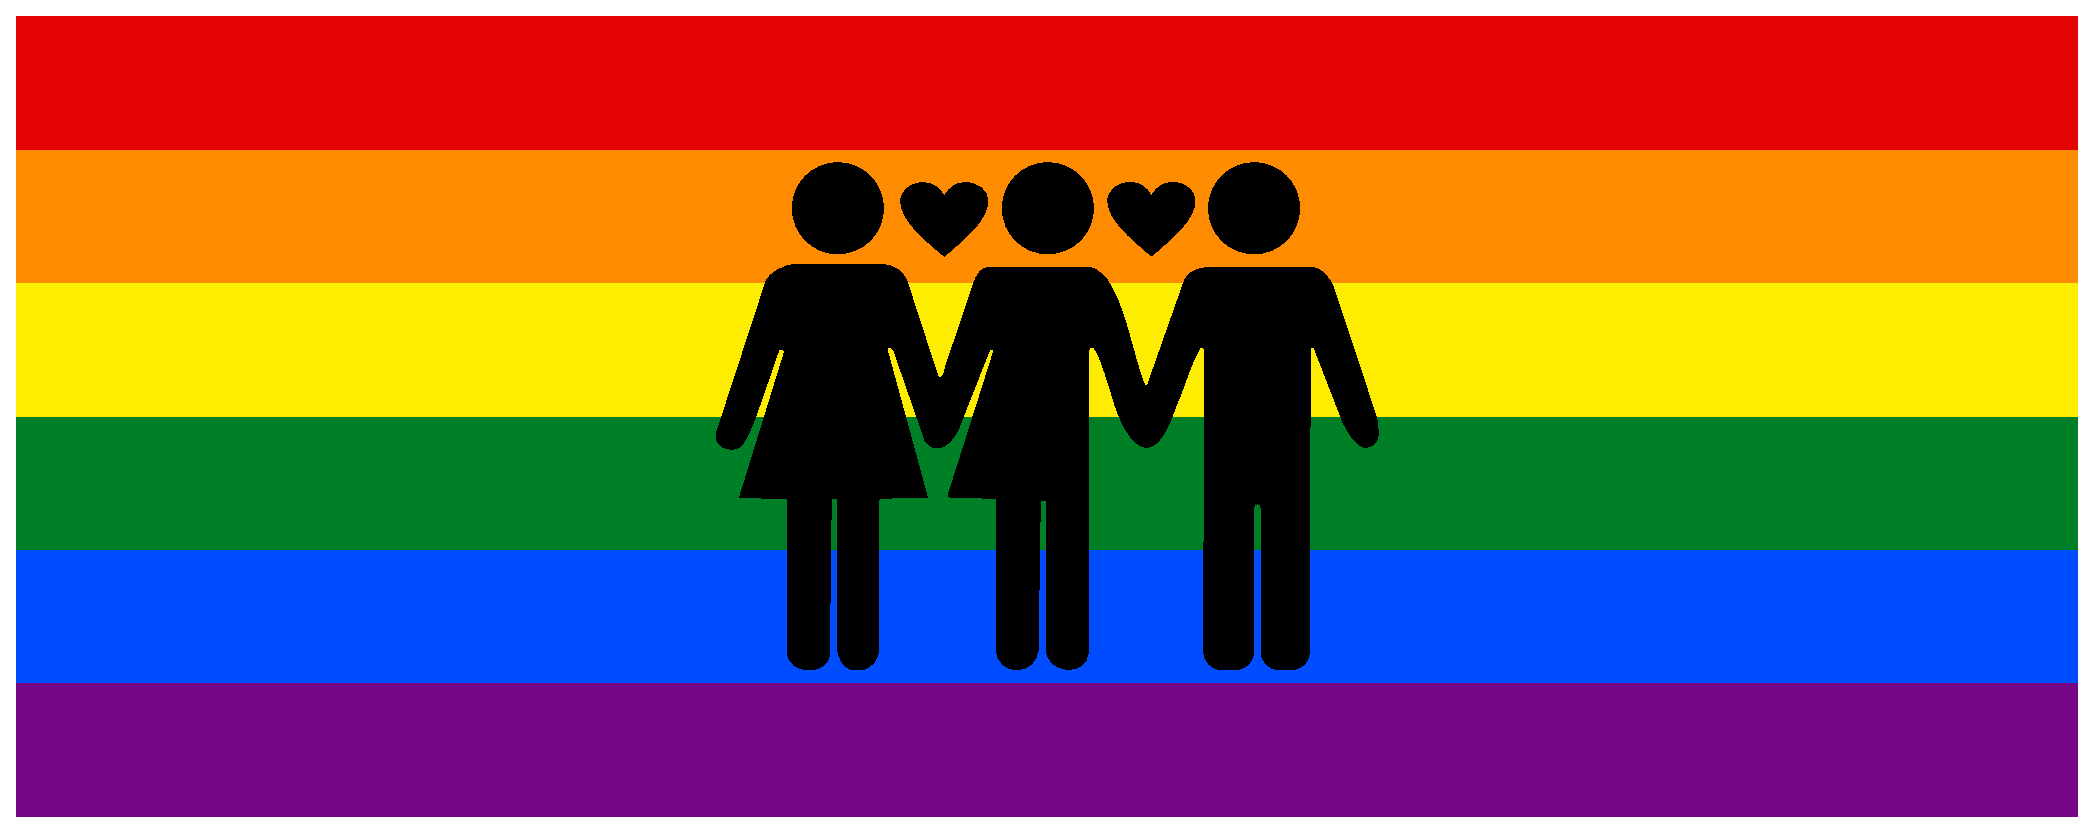
\includegraphics{polyamory.eps}} 

\vfill

\resizebox{\linewidth}{!}{היא גם לא יודעת לספור}

\vfill

~

\end{center}

\newpage

\begin{tikzpicture}
    \useasboundingbox [fill=magenta!75!white] (0,0) rectangle (\linewidth,0.5\paperheight);

	\node  at (0.5\linewidth,0.25\paperheight){
	\color{black}
	\setsize{110}
\RL{~\textbf{לא עלה תאנה ורוד!} $\raisebox{-0.25\height}{
\includegraphics[height=2ex]{figleaf.png}}$}};

\end{tikzpicture}

\vfill

\begin{center}
\setsize{70}
\color{magenta!75!white}
%מתנגדת להוורדת {\fontspec{Alef}(pinkwashing)} משטר ההפרדה הגזענית של מדינת ישראל

מתנגדת להוורדת משטר ההפרדה

הגזענית של מדינת ישראל

\vfill

\setsize{40}
\LR{\fontspec{Alef}I refuse to serve as a pink fig leaf

I oppose pinkwashing the Israeli racial segregation}

\end{center}

\vfill

~
\end{document}
